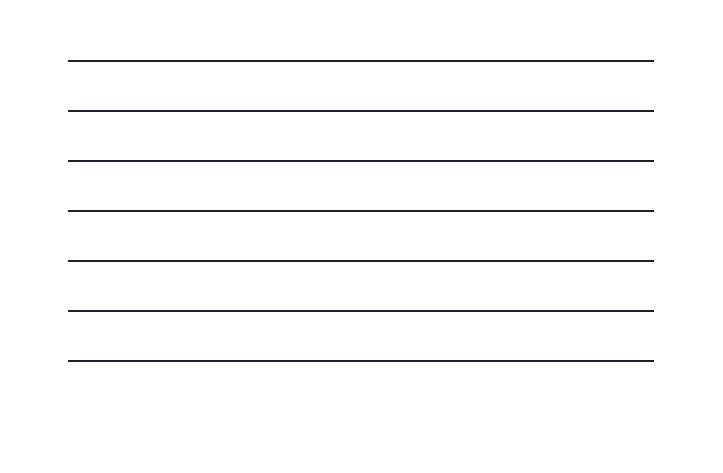
\begin{tikzpicture}[every node/.style={inner sep=0bp,outer sep=0bp}]
  \definecolor{qcA}{rgb}{0.11,0.12,0.15}
  \useasboundingbox (0bp,0bp) rectangle (240bp,150bp);
  % quiver-key: panel
  % quiver-role: series -- measured series
  % quiver-data: value = 42
  % quiver-data: value = 43
  % quiver-data: series/id = a&b
  \path[draw=qcA,line width=0.75bp] (14.4bp,138bp) -- (225.6bp,138bp);
  % quiver-key: panel
  % quiver-role: datum -- a single datum
  % quiver-data: value = 42
  % quiver-data: value = 43
  % quiver-data: series/id = a&b
  \path[draw=qcA,line width=0.75bp] (14.4bp,120bp) -- (225.6bp,120bp);
  % quiver-key: 9 starts with a digit
  % quiver-role: axis -- x axis
  % quiver-data: value = 42
  % quiver-data: value = 43
  % quiver-data: series/id = a&b
  \path[draw=qcA,line width=0.75bp] (14.4bp,102bp) -- (225.6bp,102bp);
  % quiver-key:
  % quiver-role: legend -- legend
  % quiver-data: value = 42
  % quiver-data: value = 43
  % quiver-data: series/id = a&b
  \path[draw=qcA,line width=0.75bp] (14.4bp,84bp) -- (225.6bp,84bp);
  % quiver-role: annotation -- an annotation
  % quiver-data: value = 42
  % quiver-data: value = 43
  % quiver-data: series/id = a&b
  \path[draw=qcA,line width=0.75bp] (14.4bp,66bp) -- (225.6bp,66bp);
  % quiver-role: decoration -- should not be emitted as a label
  % quiver-data: value = 42
  % quiver-data: value = 43
  % quiver-data: series/id = a&b
  \path[draw=qcA,line width=0.75bp] (14.4bp,48bp) -- (225.6bp,48bp);
  % quiver-role: other:custom role -- custom
  % quiver-data: value = 42
  % quiver-data: value = 43
  % quiver-data: series/id = a&b
  \path[draw=qcA,line width=0.75bp] (14.4bp,30bp) -- (225.6bp,30bp);
\end{tikzpicture}
